\chapter{Introduction}
\section{Objectives of this Thesis}

   
Drug injections in eye surgeries could be a very challenging task for human surgeons. Tremors and erroneous posing of the needle could lead to damages to the patient’s eyes and are not easy to prevent completely. Using an assistance robot, which provides higher precision and eliminates human errors could reduce the risks. An important task in development of the robot is to calculate the position and rotation as accurately as possible for a real-time system. An algorithm developed by Ramona Schneider, which uses OCT images, to tackle technical difficulties such as lack of available information, image noises and deformation. This allows the system to execute the calculations with great accuracy. Still there is a problem while implementing it in a real time system: The algorithm takes too much time and resources to execute. A different approach is required to accelerate the algorithm to a real-time suitable execution time. Using the same algorithm developed by Ramona, the code first needs to be restructured to utilize the full advantages of graphic cards with OpenCL, by parallelizing the code as much as possible. Furthermore, an in-depth research to understand the structure and specification of a graphic card is required to optimize the code to reach the full potential of the processing units.
    
\section{Approaches}

The main goal of Ramona’s work is to develop a reliable method to compute the position and rotation of a beveled needle. The needle can be digitally reconstructed as a point cloud by utilizing the obtained OCT images. By matching the point cloud with the CAD model, an accurate determination of rotation and position can be achieved.

Two different approaches were implemented and taken into consideration. Which are \cite{ramona}:

\begin{itemize}
	\item A developed approach for object recognition and pose estimation for rigid objects using Clustered Viewpoint Feature Histograms (CVFH) and camera roll histograms described in a paper by Aldoma et al \cite{aldoma}.

	\item A new approach similar to the Iterative Closest Point (ICP) algorithm which calculates and utilizes the direction of the needle, and then finds the rotation-shift combination along the direction with the best matched points.
\end{itemize} 

After several trials and tests it was concluded that the second approach was the best solution from the two approaches presented. The solution was also adopted in this thesis with two main objectives: Reproduction of the same accuracy, acceleration the software to an acceptable level for real time systems. Broadly speaking, the program consists of two main parts: Processing OCT images and a shifting algorithm. 

The goal of processing images is to read, analyze a set of pictures and reconstructing a needle point cloud from given input data. The important parts of this process is to remove noise, downsample OCT images, which are black and white slice captures of the needles. Figure 1.1 shows an examplary OCT image of the needle.

\begin{figure}[t!]
	\centering
	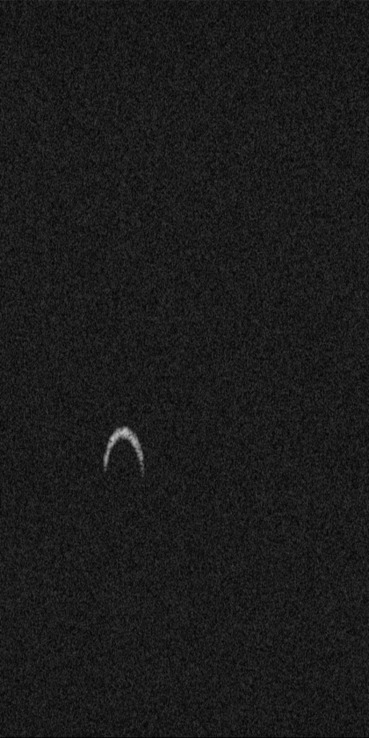
\includegraphics[width=5cm]{images/OCTimageEx.jpg}
	\caption{An examplary OCT image of the needle}
	\label{ExampleOCTImage}
\end{figure}

Whereas the white area is the actual slice of the needle. Within the scope of this thesis, only the second part, which is a quite time-consuming task, will be translated into GPU conformed code. Therefore, the focus of this thesis is the acceleration of shifting algorithm with graphic processing unit (GPU). In the next chapter a popular frame work for GPU programming will be discussed with greater details.

